\renewcommand{\documentname}{Project planning and budget overview}

\chapter{Project planning and budget overview}

So far we have discussed the theory that will function as a pillar of the software system to be developed. With this chapter we begin the sections focused on the software engineering used to define and build such a system. In this first chapter we present the planning and WBS of the software project, defining and explaining its phases, and finally showing an overview of the internal and customer budget.


\section{Planning}

The planning of the class management system, identified as Classmanager, has the following phases. They are shown with a Gantt diagram and with the WBS of the project. Due to the size of the Gantt chart, it is shown in its full version and split into phases. 

The following phases were established for the planning: \textit{Project Management}, \textit{Analysis}, \textit{Design}, \textit{Development}, \textit{Documentation}, \textit{Experiments} and \textit{Closure}.


\begin{figure}[H]
    \caption{Gantt chart}
  \centering
  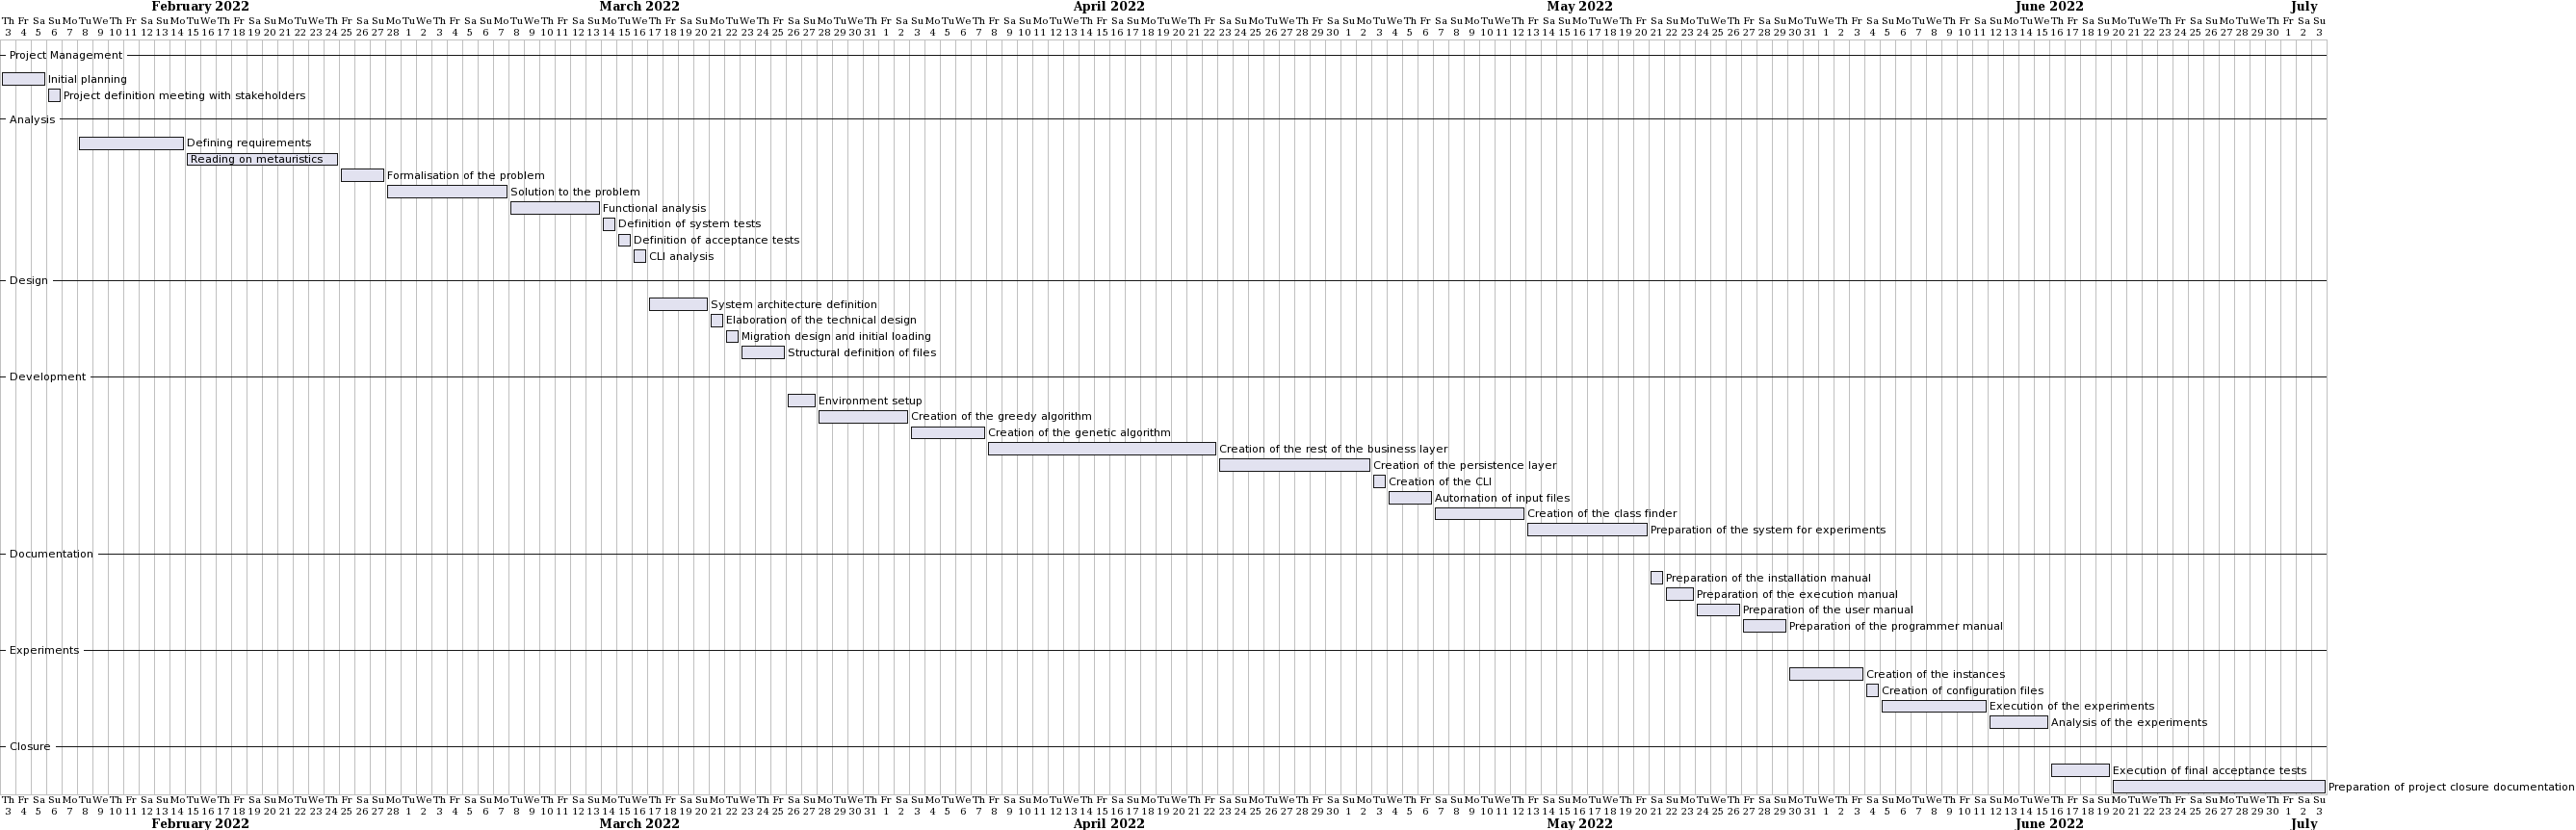
\includegraphics[scale=0.2, angle=90]{gantt.png}
\end{figure}


\subsection{Project Management}

\begin{itemize}
    \item \textbf{Initial planning}: Reading the project synopsis, first discussions with supervisors and establishing the project plan. 
    \item \textbf{Project definition meeting with stakeholders}: Requirements gathering meeting with the client, definition of objectives and scope of the project.
    \item \textbf{Project monitoring and control}: Regular meetings with supervisors and clients to discuss and review project status. 
\end{itemize}

\begin{figure}[H]
    \caption{Gantt chart: Project Management}
  \centering
  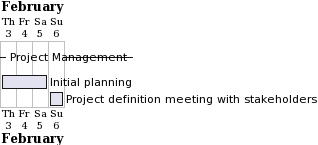
\includegraphics[scale=0.8]{gantt_01_project_management.png}
\end{figure}


\subsection{Analysis}

\begin{itemize}
    \item \textbf{Defining requirements}: Write down and review the requirements previously obtained in the meeting with the clients.
    \item \textbf{Reading on metaheuristics}: Reading diverse literature on greedy algorithms, genetic algorithms and metaheuristics. 
    \item \textbf{Formalisation of the problem}: Formal definition of the problem as an assignment problem, explaining its components and constraints.
    \item \textbf{Solution to the problem}: Theoretically elaborating the solution to the previously defined problem.
    \item \textbf{Functional analysis}: Analysis of use cases, functionality and other aspects of the software prototype.
    \item \textbf{Definition of system tests}: Tests on input files, configuration files and system functionality. 
    \item \textbf{Definition of acceptance tests}: Checking the quality of the results obtained by the system.
    \item \textbf{CLI analysis}: Study on how to run the utility and the format of its arguments. 
\end{itemize}

\begin{figure}[H]
    \caption{Gantt chart: Analysis}
  \centering
  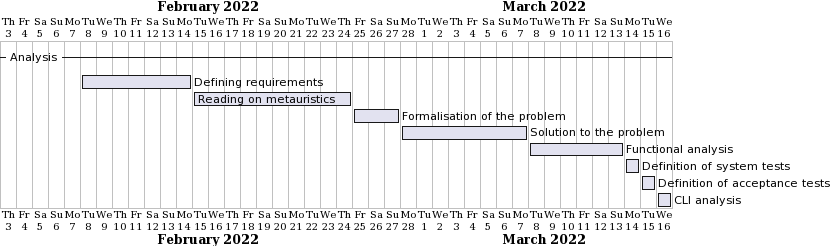
\includegraphics[scale=0.6]{gantt_02_analysis.png}
\end{figure}


\subsection{Design}

\begin{itemize}
    \item \textbf{System architecture definition}: Definition of subsystems, packages and the relationships between them.
    \item \textbf{Elaboration of the technical design}: Final class diagrams.
    \item \textbf{Migration design and initial loading}: Study on the conversion of planning and enrolment files into files with a format that can be processed by the system.
    \item \textbf{Structural definition of files}: Elaborating the final format of the input, output and configuration files. 
\end{itemize}

\begin{figure}[H]
    \caption{Gantt chart: Design}
  \centering
  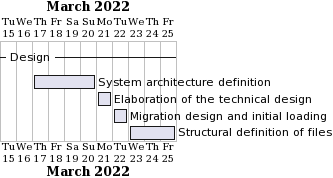
\includegraphics[scale=0.8]{gantt_03_design.png}
\end{figure}


\subsection{Development}

\begin{itemize}
    \item \textbf{Environment setup}: Creation of code and documentation repositories, configuration of text editors and tools to run and test the system.
    \item \textbf{Creation of the greedy algorithm}: Define the LCM, LFD, and the Greedy Algorithm components.
    \item \textbf{Creation of the genetic algorithm}: Define the operators of the Genetic Algorithm and its components.
    \item \textbf{Creation of the rest of the business layer}: Implement data infrastructure, log management, error handling and other business layer items. 
    \item \textbf{Creation of the persistence layer}: Develop DataAccess and file management. 
    \item \textbf{Creation of the CLI}: Utilities for all CLI content to be centralised in a single component.
    \item \textbf{Automation of input files}: Functionality of automating the files previously used by the School.
    \item \textbf{Creation of the class finder}: Functionality of searching classrooms with free time slots.
    \item \textbf{Preparations of the systems for experiments}: Adapt the system to make it easier to run many instances in parallel.
\end{itemize}

\begin{figure}[H]
    \caption{Gantt chart: Development}
  \centering
  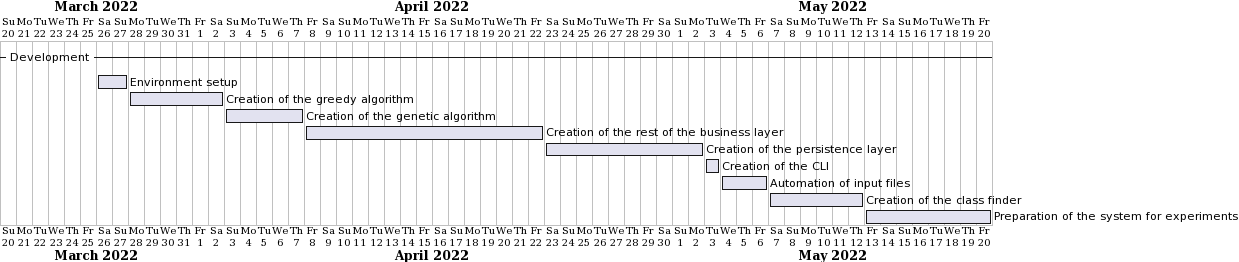
\includegraphics[scale=0.4]{gantt_04_development.png}
\end{figure}


\subsection{Documentation}

\begin{itemize}
    \item \textbf{Preparation of the installation manual}: Required dependencies and setup required to be able to run the application.
    \item \textbf{Preparation of the execution manual}: Available options for launching the software.
    \item \textbf{Preparation of the user manual}: Instructions on how to execute each functionality, explanation of how to interpret the output files and recommended configurations.
    \item \textbf{Preparation of the programmer manual}: Instructions on how to maintain the program, where to find the main parts of the code and how to interpret the log file.
\end{itemize}

\begin{figure}[H]
    \caption{Gantt chart: Documentation}
  \centering
  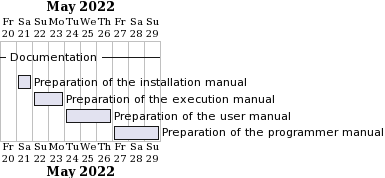
\includegraphics[scale=0.8]{gantt_05_documentation.png}
\end{figure}


\subsection{Experiments}

\begin{itemize}
    \item \textbf{Creation of the instances}: Instances are created based on actual data from past courses by using the automation functionality of the files used by the School.
    \item \textbf{Creation of configuration files}: Define the configuration files with the different combinations of values and parameters.
    \item \textbf{Execution of the experiments}: Execution of the experiments using a computer specialised in parallel runs.
    \item \textbf{Analysis of the experiments}: Analysis of the results and obtaining the best values in order to obtain the highest possible quality results.
\end{itemize}

\begin{figure}[H]
    \caption{Gantt chart: Experiments}
  \centering
  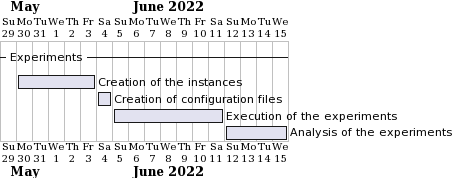
\includegraphics[scale=0.8]{gantt_06_experiments.png}
\end{figure}


\subsection{Closure}

\begin{itemize}
    \item \textbf{Execution of final acceptance tests}: Execution of tests to verify the quality of the results.
    \item \textbf{Preparation of the closure documentation}: Theoretical and technical project documentation and system manuals.
\end{itemize}

\begin{figure}[H]
    \caption{Gantt chart: Closure}
  \centering
  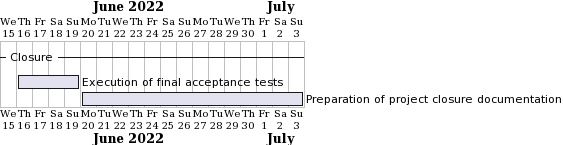
\includegraphics[scale=0.8]{gantt_07_closure.png}
\end{figure}



\section{Budget summary}

